\begin{thm}{192}{\hosi 6}{自作 DMO4th 理1}
 $x$軸上を動く点Pと、2点A$(1,1)$, B$(-1,1)$がある。$\triangle\mr{ABP}$の垂心をHとする。
 \begin{enumerate}
  \item 3点 A, B, H が鈍角三角形をなすとき、垂心Hの軌跡Lを図示せよ。
  \item Lと、線C:~$y=ax^2+bx+1$ が共有点を持つような点$(a,b)$ の範囲を図示せよ。
 \end{enumerate}
\end{thm}

\syoumon{1}
点P$(t,0)$とする。$\vvv{\mr{PA}}=(1-t, 1)$, $\vvv{\mr{PB}}=(-1-t, 1)$となる。PからABに引く垂線の式は$x=t$であるから、H$(t, h)$とおけて、$\vvv{\mr{BH}}=(t+1, h-1)$, $\vvv{\mr{AH}}=(t-1, h-1)$となる。明らかに$\vvv{\mr{PB}}\neq\vvv{0}$なので、
\[ \vvv{\mr{AH}}\cdot\vvv{\mr{PB}}=0 \quad\dou\quad \vvv{\mr{AH}}\perp\vvv{\mr{PB}} \,\,\text{または}\,\, \vvv{AH}=\vvv{0} \]
$\vvv{\mr{AH}}\neq\vvv{0}$、すなわち$t-1\neq 0$のとき、
\[ \vvv{\mr{AH}}\cdot\vvv{\mr{PB}} =-(t^2-1)+h-1=0 \,\dou\, h=t^2 \]
よって、H$(t, t^2)$~(ただし$t\neq 1$)。$t=1$の場合はP$(1,0)$で、$\angle\mr{BAH}=90^\circ$であるからHはAに一致しH$(1,1)$となるから、$t=1$でもこれは満たされる。よって、Hは曲線$y=x^2$上を動く。

$\triangle\mr{ABH}$が鈍角三角形なら、A, B, Hは一直線上にないから$t\neq 1, -1$である。このもとで鈍角三角形になるのは、
\begin{align*}
 \vvv{\mr{HA}}\cdot\vvv{\mr{HB}}&<0 & &\text{or} & \vvv{\mr{AB}}\cdot\vvv{\mr{AH}}&<0 & &\text{or} & \vvv{\mr{BA}}\cdot\vvv{\mr{BH}}&<0 \\
% \dou\quad (t^2-1)+(t^2-1)^2&<0 & &\text{or} & -2(t-1)&<0 & &\text{or} & 2(t+1)&<0 \\
 \dou\quad t^2(t^2-1)&<0 & &\text{or} & t&>1 & &\text{or} & t&<-1
\end{align*}
すなわち、$t$が$\pm1, 0$以外の実数のとき$\triangle\mr{ABH}$は鈍角三角形となる。以上より、Lは曲線$y=x^2$のうち、3点$(0,0)$, $(\pm1, 1)$を除いたもの。
\begin{figure}[H]
 \centering
 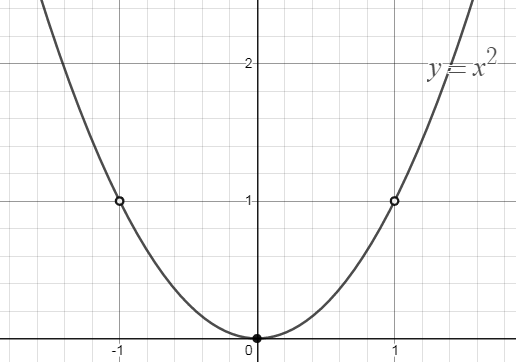
\includegraphics[width=0.6\linewidth]{../problems/Q_192/A_192_1.png}
\end{figure}

\syoumon{2}
$y=x^2$, $y=ax^2+bx+1$を連立して得る$x$の方程式$(a-1)x^2+bx+1=0$~($\cdots$ *)が、$0, \pm1$以外の実数解を持てばよい。ここで明らかに$x=0$は解にならない。

$a=1$のとき、$bx+1=0$が$\pm1$以外の解を持つために、$b\neq0, \pm1$。

$a\neq 1$のとき、(*)が実数解を持つことから、これの判別式$D$について
\[ D=b^2-4(a-1)\ge 0 \,\dou\, \frac{b^2}{4}+1\ge a \]
が必要。さらに$\pm 1$以外の解を持つためには、(*)の解が(i) $x=\pm 1$、(ii) $x=1$のみ、(iii) $x=-1$のみ、であってはならない。

(i)~この場合には(*)の左辺は$(a-1)(x^2-1)$と書けるから、
\[ (a-1)x^2+bx+1=(a-1)(x^2-1) \,\dou\, (a, b)=(0, 0) \]

(ii)~この場合には
\[ (a-1)x^2+bx+1=(a-1)(x-1)^2 \,\dou\, (a, b)=(2,-2) \]

(iii)~この場合には
\[ (a-1)x^2+bx+1=(a-1)(x+1)^2 \,\dou\, (a, b)=(2, 2) \]

以上により、求める領域は、$a\le\dfrac{b^2}{4}+1$のうち、6点$(0, 0)$, $(1, 0)$, $(1, \pm1)$, $(2, \pm2)$を除いたものとなる。
\begin{figure}[H]
 \centering
 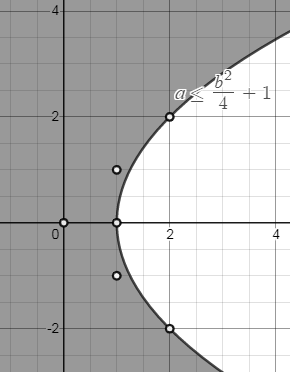
\includegraphics[width=0.6\linewidth]{../problems/Q_192/A_192_2.png}
\end{figure}
なお、境界は、除くべき点である$(1,0)$, $(2,\pm2)$以外は含める。